\documentclass[letterpaper]{article} % DO NOT CHANGE THIS
\usepackage{aaai2027}  % DO NOT CHANGE THIS
\usepackage[hyphens]{url}  % DO NOT CHANGE THIS
\usepackage{graphicx} % DO NOT CHANGE THIS
\urlstyle{rm} % DO NOT CHANGE THIS
\def\UrlFont{\rm}  % DO NOT CHANGE THIS
\usepackage{natbib}  % DO NOT CHANGE THIS AND DO NOT ADD ANY OPTIONS TO IT
\usepackage{caption} % DO NOT CHANGE THIS AND DO NOT ADD ANY OPTIONS TO IT
\frenchspacing  % DO NOT CHANGE THIS
\usepackage{amsmath}
\usepackage{booktabs}
\pdfinfo{
/TemplateVersion (2027.1)
}

\setcounter{secnumdepth}{1}

\title{Tools Help Per Question, Not on Average}
\author{Parsuram Pradhan}
\affiliations{
    parsuram.pradhan@yobytech.com
}

\begin{document}

\maketitle

\begin{abstract}
Fixed tool recipes on 150 HotpotQA and 150 Natural Questions items span 100 to 105 correct out of 300. An oracle that keeps, on each question, the better of one-shot retrieval and a six-step recipe reaches 124/300 at nearly the one-shot price. Tools help per question. They do not help as a blanket policy. The blanket result is the reward: a full tool trajectory gains about 0.03 quality and pays 0.10 in a flat action charge, against a measured dollar and latency gap of about 0.002. A 261-parameter REINFORCE policy selects one-shot retrieval whenever that charge or a large dollar weight is on, and it spends the step budget when every penalty is removed. Those selected checkpoints are one-shot retrieval on the 80{,}000-passage index. They also could not branch on the retrieval score. \(\tanh(\mathrm{score}/5)\) is 1.0 on all 300 questions, and before the first retrieval the observation is identical for every question, so the first action cannot depend on the question. On the index after the training passages are merged in (83{,}120 passages), validation selection makes the \(\lambda{=}0\) checkpoint a six-step recipe at 103/300, while \(\lambda{=}20\) and \(\lambda{=}80\) stay one-shot. Standardizing the score lets one training draw branch, 16 sequences and 103/300 at \(\lambda{=}20\). A second draw at the same seed reaches 104/300 and does not repeat that controller. \(\lambda{=}80\) stays one-shot. The gap from 100 to 124 remains open. The later rows are a different index and are not on the frozen-controller figure.
\end{abstract}

\section{Introduction}
A retrieval-augmented generator answers from passages it has fetched \cite{lewis2020rag}. An agentic loop can do more than fetch once. It can rewrite the query, retrieve again, reorder the pool, test whether the draft is supported, or stop. In a serving stack those operations do not share a price. A redundant search and a cheap reorder can look identical to a controller that sees only exact match.

Recent reinforcement-learning agents learn when to search, and they learn it for answer quality \cite{jin2025searchr1,gandhi2026grasp}. Turn count appears as an efficiency bonus. Dollars and latency do not. Open-loop routers choose a depth before they see the passages \cite{jeong2024adaptive}. Hand-written critics decide with thresholds \cite{asai2024selfrag,yan2024crag}. None of these tells a closed-loop policy when a priced tool is worth its bill.

We study that decision in a small, fully instrumented environment. The action set is frozen at retrieve, rewrite, rerank, verify, and stop. The reward is explicit: answer quality, grounding, and calibration, minus a FinOps price card, a hallucination penalty, and a per-action charge. The cost sweep uses a 261-parameter multilayer perceptron trained with REINFORCE on 100 questions and scored, frozen, on a locked set of 300. The generator, retriever, and verifier stay fixed, so a change in exact match is a change in control.

The measurements support three claims.
\begin{itemize}
\item Under the default weights, extra tools are negative expected value. A full tool trajectory gains about 0.03 quality and pays 0.10 in action charges. One-shot retrieval has the highest reward.
\item The learner follows that arithmetic. With the action charge left on, argmax evaluation is retrieve-then-stop on 300/300 questions, including when dollar and latency weights are zero. With every penalty removed, the same network spends the step budget.
\item On that 80{,}000-passage index the selected checkpoint is one-shot retrieval at every dollar weight, and each evaluation is one action string. A per-question oracle over those trajectories answers 124/300. The score feature in that run was constant, so the string could not have depended on it. Once the score feature varies, a selected checkpoint is no longer one-shot at every weight, and exact match stays inside 100 to 104.
\end{itemize}

\section{Related Work}
Retrieval-augmented generation conditions a generator on retrieved text \cite{lewis2020rag}. Agentic controllers interleave that retrieval with other tools. ReAct alternates reasoning traces and actions \cite{yao2023react}. Self-RAG learns tokens for when to retrieve and when a citation supports a sentence \cite{asai2024selfrag}. CRAG uses a retrieval evaluator to trigger a second search or a web fallback \cite{yan2024crag}. Adaptive-RAG assigns each query to no retrieval, single-step retrieval, or multi-step retrieval before any passage is observed, which makes it an open-loop contrast to a controller that can react to a bad first search \cite{jeong2024adaptive}.

Search-R1 trains the language model itself, with an outcome reward, to issue searches and reason over the results \cite{jin2025searchr1}. GRASP is the closest typed-action neighbor: a GRPO policy over semantic search, keyword search, and paragraph expansion, rewarded for answer F1, grounded reading, complementary search, and turn efficiency \cite{gandhi2026grasp}. GRASP does not price rewrite, rerank, or verification, and its efficiency term counts turns. We keep a much smaller policy and ask a prior question: once rewrite, rerank, and verify have measured dollar costs, does a learned controller spend them only when they pay?

We do not claim a comparison against a reimplementation of Search-R1, GRASP, or Adaptive-RAG on this stack. Those systems are the reason to price tools. The experiments below isolate the price.

\section{Environment and Reward}
An episode is one question. At each step the controller picks one action. The episode ends at stop, or when the step or budget cap forces a stop. The five actions are the whole interface.

\begin{itemize}
\item \textbf{Retrieve} runs BM25 \cite{robertson2009bm25} and appends the top five passages.
\item \textbf{Rewrite} asks the generator for a new query string.
\item \textbf{Rerank} reorders the current pool by lexical overlap with the query.
\item \textbf{Verify} runs a lexical natural-language-inference check of the current draft against the passages and returns support, neutral, or contradiction.
\item \textbf{Stop} emits a short answer, or abstains. Yes/no questions must be answered yes or no.
\end{itemize}

Caps are eight steps, three retrieves, two rewrites, two reranks, and two verifies. The price card meters local Qwen2.5-3B-Instruct tokens at \$0.15 and \$0.60 per million input and output tokens, BM25 at \(5\times 10^{-5}\) dollars per call, and latency at \(10^{-3}\) dollars per second scaled by a latency weight \cite{qwen2024}. Absolute dollars are an instrumentation scale for a local model. Ratios are what the policy can learn.

The observation in the cost sweep is ten numbers: tanh-scaled mean retrieval score, evidence count, remaining steps, remaining dollar budget, verifier support, verifier contradiction, and the four tool counts. There is no dataset indicator and no passage text in the control head. The generator still reads the passages. Illegal actions are masked: with no evidence the policy cannot rerank, verify, or stop. Before the first retrieval that vector is the same for every question: no evidence, a zero score, and a full budget. The question text is not an input, so the first action cannot depend on which question is being asked. Adaptivity can begin only at the second step. A later experiment replaces the tanh score with a training-slice z-score clipped to \([-3, 3]\), and it adds the top-1 score, the top-1 minus top-2 gap, a verify one-hot, and the minimum of the top five. That vector is 16-dimensional. The empty-retrieval channels stay 0, so ``we have not searched'' is not coded as a very negative score.

The terminal reward is
\begin{equation}
\begin{aligned}
R = {} & \alpha Q_{\mathrm{ans}} + \beta Q_{\mathrm{ground}} + \gamma Q_{\mathrm{cal}} \\
& - \lambda (C_{\mathrm{tok}} + C_{\mathrm{ret}}) - C_{\mathrm{lat}} \\
& - P_{\mathrm{hall}} - P_{\mathrm{act}} - P_{\mathrm{bud}} + B.
\end{aligned}
\label{eq:reward}
\end{equation}
\(Q_{\mathrm{ans}}\) is the average of exact match and token F1. \(Q_{\mathrm{ground}}\) mixes claim--evidence overlap with, on HotpotQA, recall of gold supporting titles. \(C_{\mathrm{tok}}\) and \(C_{\mathrm{ret}}\) are price-card dollars. \(C_{\mathrm{lat}}\) already includes the latency weight. \(P_{\mathrm{hall}}\) penalizes unsupported and contradicted claims, with an extra weight if verify was available and unused. \(P_{\mathrm{bud}}\) is a unit penalty if a hard budget breaks. The unused-budget bonus \(B\) is granted only when \(Q_{\mathrm{ans}} \ge 0.5\), so a cheap wrong answer does not collect an efficiency credit. The action charge is \(P_{\mathrm{act}} = \rho \max(0, n-1)\) for \(n\) actions in the episode.

Default weights are \(\alpha{=}1\), \(\beta{=}0.4\), \(\gamma{=}0.15\), \(\lambda{=}2\), latency weight \(0.5\), hallucination weight \(0.5\), and \(\rho{=}0.02\). Calibration is not a second copy of exact match. A correct answer scores \(+0.3\). Abstaining scores \(+0.6\) only when the passage list is empty, the mean retrieval score is below 3, or verify returns contradiction; any other abstention scores \(-0.2\). A wrong answer scores \(-0.4\) with evidence and \(-0.2\) without it. Abstaining on a string that already matches the gold answer scores \(-0.5\). A policy cannot farm reward by refusing whenever it would have been wrong. On the logged exams the mean-score arm of that bonus does not fire. Raw BM25 means stay above 20, and means after the lexical reranker stay above 7, so a real retrieved list never takes the \(+0.6\) path. Empty evidence and a contradiction label still do. The threshold is the same cutoff the rule policy uses for ``strong enough to rerank and verify,'' and that rule takes the strong branch on every question for the same reason.

\section{Learning}
The policy is a multilayer perceptron, \(10 \rightarrow 16 \rightarrow 5\), with 261 parameters. Width above 32 is rejected: the training slice is 100 questions. We optimize with REINFORCE \cite{williams1992reinforce}. The return is the terminal reward in Equation~\ref{eq:reward}. The baseline is an exponential moving average of that return. The entropy bonus coefficient is 0.01, the optimizer is Adam, and the learning rate is 0.003. Training reads only the 100-example training file. The evaluation file is refused by name.

At test time the action is the mode of the masked softmax. Sampling during training can visit tools that the mode never selects, so we also roll out the mode on the training questions after each epoch of the dollar sweep. The checkpoint we treat as the result is the epoch with the highest greedy training reward. It is chosen before the 300-question evaluation is opened. The last epoch is reported beside it, and it is not the selected policy when the two differ. The dollar sweep below uses this 10-dimensional head and the 100-question file. The later section trains a 16-dimensional head, 357 parameters at hidden width 16, on 500 questions, and selects the checkpoint by greedy reward on a held-out 180. Both use seed 42.

\section{Experimental Setup}
The evaluation set is locked at 300 questions: 150 HotpotQA distractor items \cite{yang2018hotpotqa} and 150 Natural Questions items \cite{kwiatkowski2019nq}. The training slice is 60 HotpotQA and 40 Natural Questions drawn from the same sources and disjoint from the evaluation ids. The shared index holds 80{,}000 passages: HotpotQA contexts, unused HotpotQA distractors, and the DPR 100-word Wikipedia passages released with Natural Questions \cite{karpukhin2020dpr,gao2022tevatron}. Gold text is a Wikipedia passage. It is not a sentence of the form ``the answer is.'' BM25 recall at five is 0.927 on HotpotQA (11 misses) and 0.587 on Natural Questions (62 misses), so a second retrieval can matter.

The generator is Qwen2.5-3B-Instruct at temperature 0 \cite{qwen2024}. The verifier is lexical, not a cross-encoder and not the generator judging itself. Three frozen controllers define the corners. One-shot retrieval fetches once and stops. The rule policy reranks and verifies when the mean BM25 score is at least 3, and it stops after verify on every question in this run. The max-tool policy spends three retrieves, one rewrite, one rerank, and one verify. Reward-weight ablations that keep this rule policy fixed are a scoring check: exact match does not move, and only the scalar does. Every learned number below is a frozen argmax pass over the same 300 questions. We report one seed (42). Table~\ref{tab:frozen}, Table~\ref{tab:learned}, and Figure~\ref{fig:frontier} are this 80{,}000-passage index. Merging the 500 training and 180 validation passages into the corpus changes BM25 for the locked 300 as well. The later section reports that 83{,}120-passage index only against retrieve-then-stop from the same run. Those rows are not added to Table~\ref{tab:frozen}.

\section{Results}

\begin{figure*}[t]
\centering
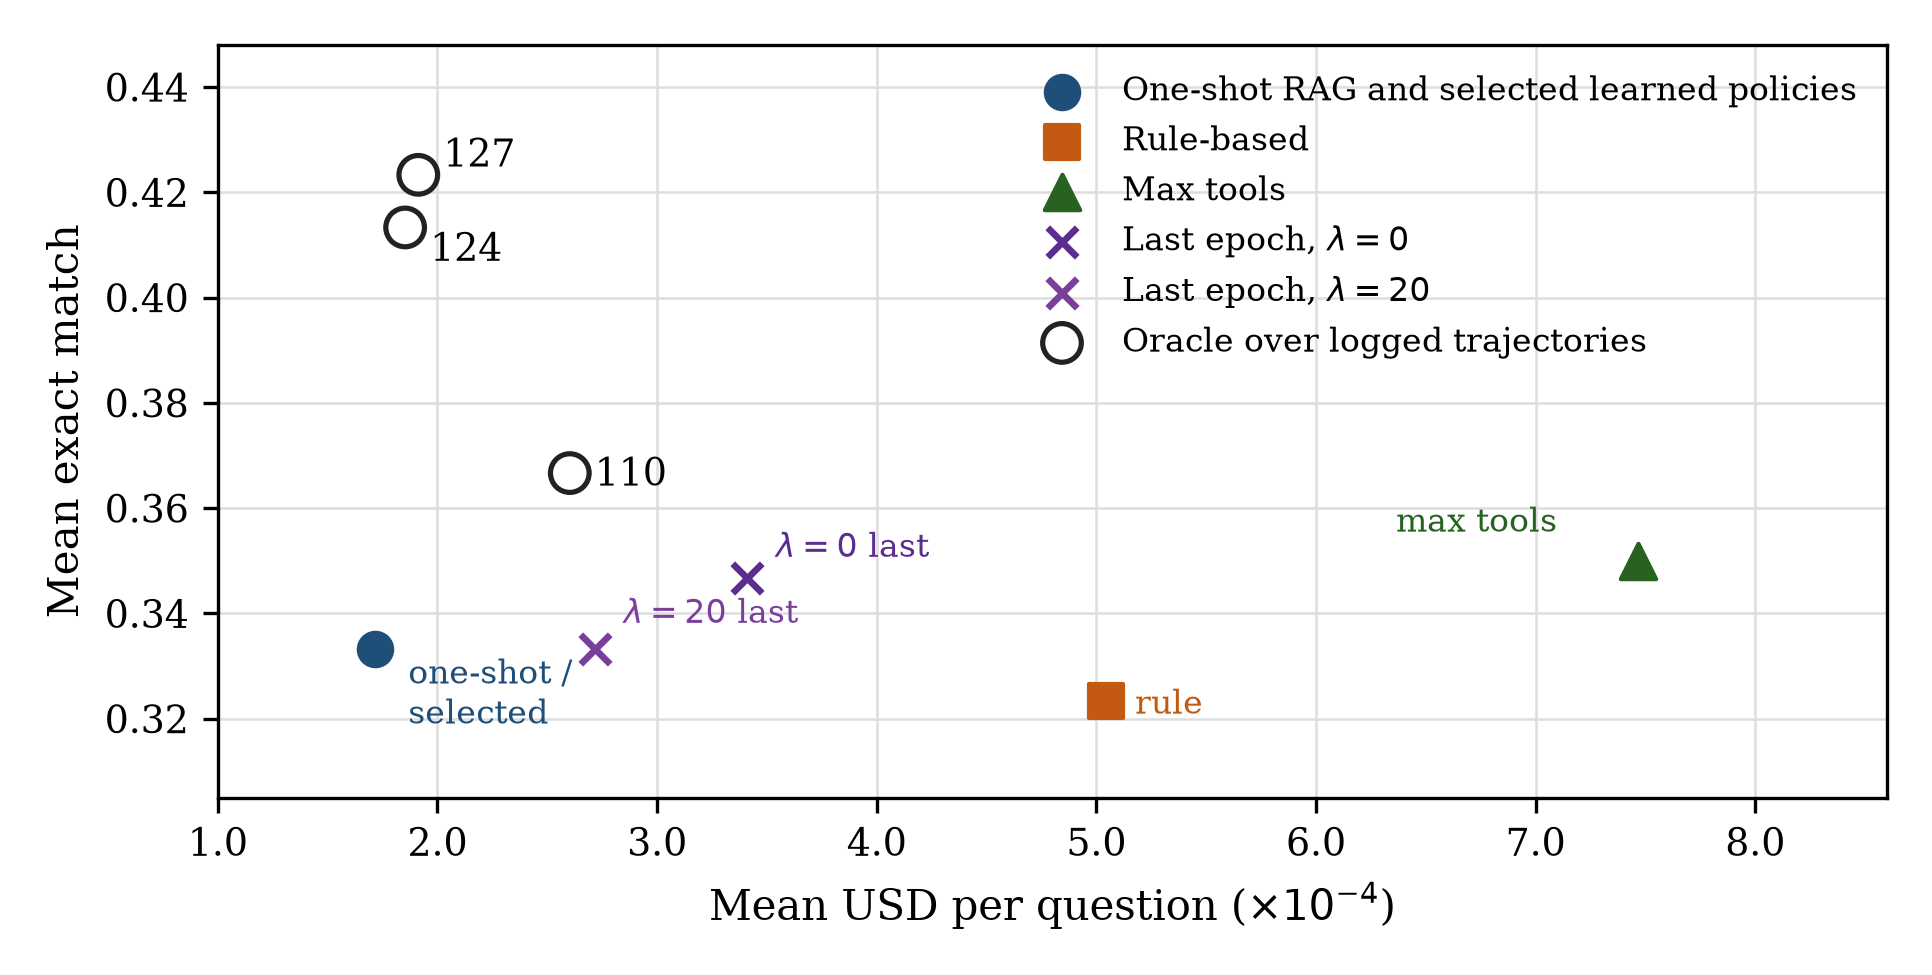
\includegraphics[width=0.92\textwidth]{figures/frontier.png}
\caption{Exact match against mean dollars per question, on the 80{,}000-passage index only. Squares are frozen controllers. The filled circle is every selected learned checkpoint from the dollar sweep; all three sit on one-shot retrieval. Crosses are last-epoch recipes that the training reward did not select. Hollow circles are oracles over trajectories logged on this same index, not learned policies: 110 uses one-shot retrieval on HotpotQA and the zero-dollar recipe on Natural Questions; 124 keeps the better of those two answers on each question; 127 may also use the max-tool trajectory. Checkpoints from the 83{,}120-passage index are omitted.}
\label{fig:frontier}
\end{figure*}

\subsection{Extra Tools Buy Five Answers}
Table~\ref{tab:frozen} splits the frozen controllers by dataset. Overall exact match is a mix of a multi-hop slice near 0.39 and a single-hop slice near 0.28, so we do not rank policies by the pooled number alone.

\begin{table*}[t]
\centering
\setlength{\tabcolsep}{4pt}
\begin{tabular}{lrrrrrrr}
\toprule
Policy & Hotpot & NQ & EM & Correct & \$ & Steps & Reward \\
\midrule
One-shot & 59/150 & 41/150 & 0.333 & 100/300 & \(1.72\times 10^{-4}\) & 2 & 0.580 \\
Rule & 56/150 & 41/150 & 0.323 & 97/300 & \(5.04\times 10^{-4}\) & 4 & 0.531 \\
Max tools & 61/150 & 44/150 & 0.350 & 105/300 & \(7.47\times 10^{-4}\) & 7 & 0.509 \\
\bottomrule
\end{tabular}
\caption{Frozen controllers on the 300-question evaluation, 80{,}000-passage index. Hotpot is HotpotQA exact-match count. NQ is Natural Questions. EM and reward are means. One-shot retrieval has the highest reward. The max-tool policy has the highest exact match.}
\label{tab:frozen}
\end{table*}

The max-tool policy recovers a net of two HotpotQA answers and three Natural Questions answers over one-shot retrieval, and its overall token F1 rises from 0.397 to 0.422. Mean cost rises by a factor of about 4.3, from \(1.72\times 10^{-4}\) to \(7.47\times 10^{-4}\) dollars, and mean latency from about 1.0\,s to 3.4\,s. Reward falls from 0.580 to 0.509.

The components say why. From one-shot retrieval to the max-tool policy, \(Q_{\mathrm{ans}}\) rises by 0.021 (0.365 to 0.386), \(Q_{\mathrm{ground}}\) by 0.018 (0.647 to 0.665), and \(Q_{\mathrm{cal}}\) by 0.009 (\(-0.137\) to \(-0.128\)). With the default weights that is a quality gain of \(0.030\). The action charge rises from 0.02 to 0.12. Scaled dollars and latency together rise by about 0.002. A quality term of 0.03 against a charge of 0.10 is a reward loss of about 0.07, which matches the observed gap. Of the penalty that separates the two trajectories, about 99 percent is \(\rho\) and about 1 percent is the price card. One extra retrieval costs roughly \(3\times 10^{-4}\) in the \(\lambda{=}2\) dollar term and 0.02 in \(\rho\), so the flat charge is about sixty times the measured dollar price of that call. The rule policy, which always pays for a rerank and a verify, lands between them on both cost and reward and does not improve exact match.

On a stratified 100-question rescore of the same rule trajectories, exact match stays 0.34. Answer-only reward is 0.362, adding grounding raises it to 0.547, and the full default objective scores 0.499. The weights change the scalar. They do not change a frozen controller.

\subsection{The Learner Follows the Charge}
Table~\ref{tab:learned} is the learned policy under objectives that turn pieces of Equation~\ref{eq:reward} off. The network is the same size in every row.

\begin{table*}[t]
\centering
\setlength{\tabcolsep}{3.5pt}
\begin{tabular}{llrrl}
\toprule
Objective & Checkpoint & EM & Correct & Action string \\
\midrule
Default, \(\rho{=}0.02\), \(\lambda{=}2\) & 5 epochs & 0.333 & 100/300 & retrieve, stop \\
\(\lambda{=}\mu{=}0\), \(\rho{=}0.02\) & 5 epochs & 0.333 & 100/300 & retrieve, stop \\
Answer only & 5 epochs & 0.340 & 102/300 & cap: 3 retrieve, 2 rewrite, 2 verify \\
\(\lambda{=}0\), \(\rho{=}0\) & best, epoch 25 & 0.333 & 100/300 & retrieve, stop \\
\(\lambda{=}0\), \(\rho{=}0\) & last, epoch 40 & 0.347 & 104/300 & 1 retrieve, 2 rewrite, 2 verify \\
\(\lambda{=}20\), \(\rho{=}0\) & best, epoch 15 & 0.333 & 100/300 & retrieve, stop \\
\(\lambda{=}20\), \(\rho{=}0\) & last, epoch 40 & 0.333 & 100/300 & retrieve, retrieve, retrieve, stop \\
\(\lambda{=}80\), \(\rho{=}0.02\) & best \(=\) last & 0.333 & 100/300 & retrieve, stop \\
\bottomrule
\end{tabular}
\caption{Frozen argmax evaluation of the learned policy. Each row is one action string on all 300 questions. The selected checkpoint is the best greedy reward on the 100 training questions. Answer only removes every penalty, including \(\rho\). The \(\lambda{=}20\) last epoch repeats the same BM25 call three times.}
\label{tab:learned}
\end{table*}

Under the default objective the training samples still use tools: over five epochs, mean training steps stay near 4 and mean verify calls stay between 0.39 and 0.55. The mode does not. Argmax evaluation is retrieve-then-stop on 300/300 questions, with the same predictions as one-shot retrieval. Entropy during training hid a retrieve-then-stop mode.

Zeroing dollar and latency weights, while leaving \(\rho{=}0.02\), does not move that mode. The training curve still samples tools. The evaluation is again retrieve-then-stop, with identical predictions. The price card is not what pins the policy.

Removing every penalty does move it. Trained only on \(Q_{\mathrm{ans}}\), the mode uses all eight steps on 300/300 questions: three retrieves, two rewrites, and two verifies. Exact match rises from 100/300 to 102/300 (HotpotQA 60/150, Natural Questions 42/150), with 9 recoveries and 7 regressions. The trainer can leave two steps. It does so when extra steps cannot lower the return.

Figure~\ref{fig:frontier} and the last five rows of Table~\ref{tab:learned} place the dollar weight on either side of the quality gap. At \(\lambda{=}80\), the extra max-tool dollars are about \(80 \times 5.8\times 10^{-4} \approx 0.046\), which is larger than the 0.03 quality those tools buy, and \(\rho\) is also on. Greedy training is retrieve-then-stop on all 40 epochs, and so is the evaluation. At \(\lambda{=}20\) and \(\rho{=}0\), the same extra dollars cost about 0.012 and are still smaller than 0.03, so untargeted tools are positive expected value on the frozen gap. The selected checkpoint, epoch 15, is retrieve-then-stop. The last epoch retrieves three times and stops. The three calls return the same passage ids, the answers match one-shot retrieval on 300/300 questions, and the spend rises from \(1.72\times 10^{-4}\) to \(2.72\times 10^{-4}\) dollars. At \(\lambda{=}0\) and \(\rho{=}0\), tools are free. The selected checkpoint is again epoch 25, retrieve-then-stop, training exact match 0.43. The last epoch is a six-step recipe---one retrieve, two rewrites, two verifies---with training exact match 0.40 and evaluation exact match 0.347 (104/300). On the training questions that recipe is three answers worse. On the evaluation set it is four answers better, and the split is uneven: HotpotQA falls from 59/150 to 53/150 while Natural Questions rises from 41/150 to 51/150. We do not treat 0.347 as the selected result. The selection rule, fixed before looking at the 300, returns one-shot retrieval.

\subsection{Constant Recipes Leave a Per-Question Gap}
Every learned evaluation in Table~\ref{tab:learned} uses one action sequence on all 300 questions. That description is accurate for these checkpoints, and it is not evidence that the controller looked at the score and declined to use it. The only score input in this 10-dimensional observation is \(\tanh\) of the mean BM25 score divided by 5. Top-1 BM25 on this corpus runs from about 26 to 122, median about 49, so the feature is 1.0 on all 300 questions. The policy could not branch on a constant.

The verifier is not vacuous. On the rule policy's trajectories it returns 14 contradictions, 31 neutrals, and 105 supports on HotpotQA, and 0 contradictions, 18 neutrals, and 132 supports on Natural Questions. The next action after verify is stop on 300/300 questions. The zero-dollar last epoch does call verify. Its final labels are 14 contradictions, 55 neutrals, and 231 supports. After a non-supporting label the next action is a second verify or stop, never a new retrieval or rewrite. Flipping the contradiction bit on a real post-verify observation changes action probabilities by at most 0.0068, and the mode stays verify either way. The first action is under a stronger constraint than the score. At step zero the observation is identical across the 300 questions, so that action is one choice for the whole evaluation. Anything that depends on the question has to wait until the second step, after a retrieval has been observed.

Against one-shot retrieval, that six-step recipe repairs 6 HotpotQA answers and breaks 12, and repairs 18 Natural Questions answers and breaks 8. The net is \(+4\). An oracle that keeps the better answer on each question scores 124/300 at a mean cost of \(1.85\times 10^{-4}\) dollars, close to one-shot retrieval, because it pays for the long trajectory only where the answer changes. Restricting the oracle to one-shot retrieval on HotpotQA and the six-step recipe on Natural Questions scores 110/300 at \(2.60\times 10^{-4}\) dollars, about a third of the max-tool bill. Allowing the max-tool trajectory as a third option scores 127/300. Single policies on this index span 100 to 105 correct. The 24-answer gap from 100 to 124 is the room a controller has if it reads the question in front of it. A dataset bit would be enough for the jump to 110, and the observation does not contain one. The jump to 124 requires a per-question choice. The policies in Table~\ref{tab:learned} do not make that choice. The ceilings 110, 124, and 127 are this index. They are not reused for the next section.

\subsection{A Score the Policy Can Read}
The next runs add the 500 training questions and 180 validation questions to the corpus, so the index holds 83{,}120 passages. Retrieve-then-stop on that index scores 100/300, HotpotQA 60/150 and Natural Questions 40/150, at \(1.72\times 10^{-4}\) dollars. Twenty of the 300 questions change their top passage relative to Table~\ref{tab:frozen}, which is why that table's one-shot row is HotpotQA 59 and Natural Questions 41. A learned row below is compared only with retrieve-then-stop from the same run.

Validation selection, still on the saturated tanh score, changes which checkpoint is one-shot. The \(\lambda{=}0\) checkpoint with the best greedy reward on the 180 is one six-step recipe on all 300 questions: retrieve, rewrite, rewrite, retrieve, retrieve, stop. It scores 103/300 (HotpotQA 60/150, Natural Questions 43/150) at \(4.21\times 10^{-4}\) dollars. The \(\lambda{=}20\) and \(\lambda{=}80\) selected checkpoints are retrieve-then-stop, 100/300. ``The selected checkpoints are one-shot retrieval'' is true here for \(\lambda{=}20\) and \(\lambda{=}80\). It is false for \(\lambda{=}0\). The recipe is still one string. The score channel it was given could not support a branch. Those trajectories are kept in the repository history. The files on disk under the same names are the z-scored retraining.

Standardizing the four score channels, and training again at seed 42, is the first run in which the policy can see the score. The selected \(\lambda{=}20\) checkpoint emits 16 action sequences, scores 103/300 (HotpotQA 59/150, Natural Questions 44/150) at \(5.31\times 10^{-4}\) dollars, and against this run's retrieve-then-stop is \(+8\) answers and \(-5\). A threshold on the decision-time mean score at 45.7 reproduces 278 of 300 decisions at the second step, which is the first step that can see a retrieval: weaker retrieval is rewritten, stronger retrieval is searched again. The selected \(\lambda{=}0\) checkpoint scores 100/300 with two sequences, spends about two verifies per question, and changes 0 of 300 predictions relative to retrieve-then-stop, at \(3.11\times 10^{-4}\) dollars. \(\lambda{=}80\) is retrieve-then-stop on every greedy epoch.

A second training run, same config, same seed, new output files, does not repeat that controller. The selected \(\lambda{=}0\) and \(\lambda{=}20\) checkpoints tie at 104/300 (HotpotQA 60/150, Natural Questions 44/150) and agree on the 300 answers. \(\lambda{=}20\) is one six-step recipe on 270 of 300 questions, at \(4.14\times 10^{-4}\) dollars, and that recipe holds the whole gain over retrieve-then-stop (\(+9 / -5\), union 109/300). \(\lambda{=}0\) uses 15 sequences and two verifies, at \(5.37\times 10^{-4}\) dollars, and those verifies change 0 answers relative to the \(\lambda{=}20\) checkpoint. \(\lambda{=}80\) is again retrieve-then-stop, and its predictions match the previous \(\lambda{=}80\) file on 300/300 questions. Best exact match moves from 103 to 104, one answer. The fact that repeated is the failure of \(\lambda{=}80\) to leave one-shot retrieval, which the dollar arithmetic already required. The fact that did not repeat was the 16-sequence controller.

Table~\ref{tab:zscore} collects the selected checkpoints. Naive retrieval, the rule policy, and the max-tool policy have not been rerun on this index, so the table has no frozen squares and no rebuilt 124. Until that pilot is scored, Figure~\ref{fig:frontier} stays the 80{,}000-passage figure.

\begin{table*}[t]
\centering
\setlength{\tabcolsep}{4pt}
\begin{tabular}{llrrrr}
\toprule
Run & Selected checkpoint & Correct & Sequences & Steps & \$ \\
\midrule
15-d, tanh score & \(\lambda{=}0\) & 103/300 & 1 & 6.00 & \(4.21\times 10^{-4}\) \\
15-d, tanh score & \(\lambda{=}20\) and \(\lambda{=}80\) & 100/300 & 1 & 2.00 & \(1.72\times 10^{-4}\) \\
16-d, z-score, draw 1 & \(\lambda{=}20\) & 103/300 & 16 & 7.49 & \(5.31\times 10^{-4}\) \\
16-d, z-score, draw 1 & \(\lambda{=}0\) & 100/300 & 2 & 3.97 & \(3.11\times 10^{-4}\) \\
16-d, z-score, draw 1 & \(\lambda{=}80\) & 100/300 & 1 & 2.00 & \(1.72\times 10^{-4}\) \\
16-d, z-score, draw 2 & \(\lambda{=}0\) & 104/300 & 15 & 7.65 & \(5.37\times 10^{-4}\) \\
16-d, z-score, draw 2 & \(\lambda{=}20\) & 104/300 & 6 & 5.89 & \(4.14\times 10^{-4}\) \\
16-d, z-score, draw 2 & \(\lambda{=}80\) & 100/300 & 1 & 2.00 & \(1.72\times 10^{-4}\) \\
\bottomrule
\end{tabular}
\caption{Selected checkpoints on the 83{,}120-passage index. Retrieve-then-stop on this index is 100/300 at \(1.72\times 10^{-4}\) dollars. Draw 1 and draw 2 are two training runs at seed 42. Sequences is the number of distinct action strings on the 300. These rows are not comparable to Table~\ref{tab:frozen}.}
\label{tab:zscore}
\end{table*}

\section{Limitations}
The policy never reads passage text, so this is a study of the reward and of credit assignment in a compact controller, not of GRPO fine-tuning of the generator. The cost sweep is one training run at seed 42 on 100 questions, with a 261-parameter head. The later section is two training runs at the same seed, on 500 questions, with a 357-parameter head. The frozen controllers are deterministic at temperature zero, so the seed applies to the learned rows and not to Table~\ref{tab:frozen}. We report no standard deviation. With two draws, the honest summary is the pair of values: best exact match is 103 and then 104, and the 16-sequence controller appears in the first draw only. Both draws used seed 42, so they are not a seed sweep. The planned final run, if the compute budget allows, is three fresh trainings at seeds 42, 43, and 44, reported as the three values or as a min--max range. Seeds multiply training only. Naive retrieval, the rule policy, and the max-tool policy do not need a seed.

Two indexes appear in this paper, and they are not mixed in one table. Table~\ref{tab:frozen}, Table~\ref{tab:learned}, and Figure~\ref{fig:frontier} are 80{,}000 passages. Table~\ref{tab:zscore} is 83{,}120. The frozen controllers and the 110 / 124 / 127 ceilings have not been rebuilt on the larger index. The 15-dimensional trajectories are in the repository history; the files on disk with those names are the z-scored retraining.

The claims a seed cannot flip are narrower than a first draft of this paper stated. Argmax evaluation is retrieve-then-stop whenever the action charge is on, and whenever \(\lambda{=}80\). A single action string on all 300 questions is a property of the saturated 10-dimensional run, and of \(\lambda{=}80\) after the score was fixed. It is not a property of the selected \(\lambda{=}0\) and \(\lambda{=}20\) checkpoints in Table~\ref{tab:zscore}. The per-question oracle of 124 is a statement about the 80{,}000-passage trajectories. The first action is identical across questions in every run, because the observation at step zero does not contain the question. The verifier and the reranker are lexical. The price card's absolute level is a local-model scale; the finding is the ratio of \(\rho\) to that scale. A neural verifier, a dense retriever, or a generator-sized policy could change the 0.03 quality gap, which would move the break-even dollar weight. We did not run that comparison. Adaptive-RAG and GRASP remain external reference points, not rows in Table~\ref{tab:frozen}.

\section{Conclusion}
Tools help per question. On the 80{,}000-passage index, fixed recipes span 100 to 105 correct, and an oracle over trajectories already in hand answers 124 of 300 at nearly the one-shot price, because it pays for the long trajectory only where the answer changes.

The flat action charge explains the average. A full tool trajectory buys about five exact-match answers and pays about 0.10 in action charges, against a measured dollar and latency gap of about 0.002. On that index, the checkpoints selected by greedy training reward are one-shot retrieval at every dollar weight we tried. The same trainer spends the step budget when every penalty is removed. Those policies could not branch on the retrieval score: the feature was constant, and the first action is taken before any question-specific observation exists.

Once the score is standardized, the selected \(\lambda{=}0\) and \(\lambda{=}20\) checkpoints leave one-shot retrieval. The first draw's \(\lambda{=}20\) checkpoint uses 16 action sequences. The second draw branches as well, on a different controller, and exact match stays at 103 or 104. \(\lambda{=}80\), and every run with the action charge left on, remains one-shot retrieval. Closing the gap from 100 to 124 requires a controller that repeats on a second training run, trained against an objective in which a useful tool call is cheaper than the answer it buys, and scored on one index. The frozen baselines on the 83{,}120-passage index are not in this paper yet.

\section*{Ethical Statement}
A cost term can be satisfied by refusing to answer. The calibration scores penalize abstention when passages are already in hand, and they penalize a confident wrong answer more than an answer with no evidence. On this corpus the arm that pays \(+0.6\) for a mean score below 3 does not fire, so that bonus is not a path the logged policies can take. The checkpoints selected under the default action charge match one-shot retrieval, including its errors, and they never call the verifier. Later checkpoints that spend tools change only a handful of answers and, on the paths where verify runs for every question, do not turn a contradiction into a new retrieval. Deploying either behavior would ship unsupported answers. We report the failure and do not present these checkpoints as a serving policy.

\bibliography{references}

\end{document}
